% This is a LaTeX thesis template for University of Sydney.
% to be used with Rmarkdown
% Emi Tanaka is responsible for this modified template.
% The original template is by Rob J Hyndman for students in Monash University.
% Version: 28 July 2018

\documentclass{sydneythesis}

%%%%%%%%%%%%%%%%%%%%%%%%%%%%%%%%%%%%%%%%%%%%%%%%%%%%%%%%%%%%%%%
% Add any LaTeX packages and other preamble here if required
%%%%%%%%%%%%%%%%%%%%%%%%%%%%%%%%%%%%%%%%%%%%%%%%%%%%%%%%%%%%%%%

\author{Bharvi Dhall}
\title{Single cell RNA-Sequencing and co-expression analysis for determination
of highly variable genes and to identify senecence associated profiles}
\degrees{}
\def\country{Ireland}
\def\department{School of Mathematics and Statistics}
\def\university{Maynooth University}
\def\degreetitle{Masters Degree}
\def\logo{download.png}
% Add subject and keywords below
\hypersetup{
     pdfsubject={},
     pdfkeywords={statistics},
     pdfauthor={Bharvi Dhall},
     pdftitle={Single cell RNA-Sequencing and co-expression analysis for determination
of highly variable genes and to identify senecence associated profiles},
     pdfproducer={Bookdown with LaTeX}
}


\bibliography{thesisrefs}

\usepackage{float}

\usepackage{verbatim}

\usepackage{hyperref}

\usepackage{url}

\usepackage[bottom]{footmisc}


\begin{document}

\titlepage

\pagenumbering{roman}

\tableofcontents
\cleardoublepage

\listoffigures
\cleardoublepage

\listoftables
\cleardoublepage

{\setstretch{1.2}\sf\tighttoc\doublespacing}

\chapter*{Preface}\label{preface}
\addcontentsline{toc}{chapter}{Preface}

The abstract is a summary of the whole thesis. Typically this section
would have about 250-350 words. Check the rules of your School or
University.

\pagenumbering{gobble}

\chapter*{Acknowledgement}\label{acknowledgement}
\addcontentsline{toc}{chapter}{Acknowledgement}

The abstract is a summary of the whole thesis. Typically this section
would have about 250-350 words. Check the rules of your School or
University.

\pagenumbering{gobble}

\chapter*{Abstract}\label{abstract}
\addcontentsline{toc}{chapter}{Abstract}

The abstract is a summary of the whole thesis. Typically this section
would have about 250-350 words. Check the rules of your School or
University.

\clearpage\pagenumbering{arabic}\setcounter{page}{0}

\chapter*{Table of Contents}\label{table-of-contents}
\addcontentsline{toc}{chapter}{Table of Contents}

\clearpage\pagenumbering{arabic}\setcounter{page}{0}

\chapter*{List of figures}\label{list-of-figures}
\addcontentsline{toc}{chapter}{List of figures}

The abstract is a summary of the whole thesis. Typically this section
would have about 250-350 words. Check the rules of your School or
University.

\chapter*{List of tables}\label{list-of-tables}
\addcontentsline{toc}{chapter}{List of tables}

The abstract is a summary of the whole thesis. Typically this section
would have about 250-350 words. Check the rules of your School or
University.

\chapter*{Nomenclature}\label{nomenclature}
\addcontentsline{toc}{chapter}{Nomenclature}

The abstract is a summary of the whole thesis. Typically this section
would have about 250-350 words. Check the rules of your School or
University.

\chapter{INTRODUCTION}\label{introduction}

\section{Purpose and Motivation}\label{purpose-and-motivation}

Cell is the basic structural unit of life and human body is made up of
millions of cells which are responsible for carrying out various
functions and life processes. With time, these processes in the human
body begin to depreciate and become inefficient, thereby causing
sickness and impacting the health of human beings. Therefore, it is
important to study and analyse various aspects of human body to keep
human population healthy and make it resistant to diseases.

In early centuries, the health care system was more of a sick-cure
system where a person was cured once he got any illness. With
advancement in healthcare and medicine this approach has now been
shifted to detect the cause of underlying disease instead to make our
health care system disease proof. Identification of
senescence-associated transcriptional profiles is one such example.

This thesis involves the analysis of two RNA sequencing datasets namely
liver and bone marrow. This project aims to reduce the number of genes
with the help of various dimensionality reduction techniques, to find
differentially expressed genes and thus investigating the genes that are
associated with cellular senescence.The scope of the project also
extends to perform gene co-expression analysis to find which genes are
correlated with those differentially expressed genes. Differential gene
expression analysis is also carried out to test if there are any
significant differences in gene expressions between different
conditions.

****Describe one line about each chapter

\section{Biological Background}\label{biological-background}

We all know that cell is the basic structural unit of all living
organisms and human body consists of trillions of cells, and these cells
have specialised functions which are responsible for healthy functioning
of different organs. The nucleus of cell contains sub-cellular
structures known as chromosomes which are responsible for transferring
genetic material. Each chromosome has tightly packed DNA. Information
stored in DNA is used to synthesize a protein which is responsible for
functioning of a cell. Gene is a part of DNA on chromosome which is
transcribed to RNA, which is then translated to amino acids which get
folded to synthesise proteins. This process of synthesizing proteins
from DNA is known as gene expression \autocite{crick1970central} .

\begin{figure}

{\centering 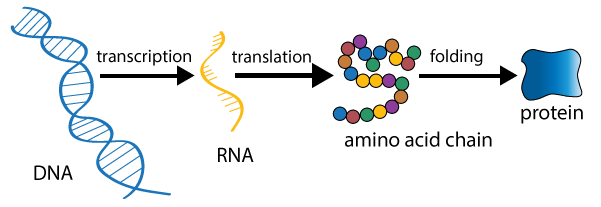
\includegraphics[width=8.35in]{Figure-1} 

}

\caption{Gene Expression-Conversion of DNA to Protein}\label{fig:unnamed-chunk-2}
\end{figure}

Note: This image has been downloaded
from:\url{http://bio.academany.org/2017/labs/BioRiiDL_2017/sreejith/images/assignments/dogma.png}

The knowledge of gene expression helps us to find and target various
problems in human body as mutation of cells cause diseases and we can
study the difference in normal and mutated cells by their gene
expression.

Cells can accomplish diverse functions with identical DNA in part by
controlling the quantity of RNA which is produced from each gene. For
example, although cells throughout the human body have essentially the
same DNA, of all genes only some specific genes are turned on which
leads to different appearances of the cell \autocite{schug2005promoter},
thereby allowing tissues to perform diverse functions.

The activity of thousands of genes is measured at once to create a
global picture of functioning in cells. This is known as expression
profiling \autocite{metsis2004whole}. This is done to find out which
cells are actively dividing or how these cells are reacting to a
treatment. The data required for carrying out such analysis is generated
using various Transcriptomics
technologies\autocite{lowe2017transcriptomics} like DNA-Microarrays and
RNA-Sequencing. In this project, we will be using RNA-Sequencing data
for analysing the genes associated with cellular senescence.

Cellular senescence is the phenomenon associated with ageing of cells
due to which cells are no longer able to divide and this can occur
because of damaged DNA \autocite{hayflick1961serial}.Normal cells in our
body grow,repair,replicate and die whereas senescent cells cease to
divide and often lead to loss of function and are found in organs with
chronic diseases.Study of senescent cells is an undiscovered and
fascinating topic in the field of biotechnology and immunology as
removal of senescent cells from the human body may slow down or reverse
ageing \autocite{de2017fountain}. Presence of senescent cells when
tested on mice lead to physical dysfunction whereas the removal of these
cells extended their lifespan and restored health
\autocite{pan2017inhibition}.

\section{Dataset Description and
availability}\label{dataset-description-and-availability}

The datasets used in this project are generated using scRNA-Seq. ScRNA
is a detailed study if geneexpression as it tries to capture the
activity of thousands of genes in a single cell.It has provided a lot of
useful insights in the field of cancer
genomics\autocite{hwang2018single} and is a new domain with ongoing
research.Sc RNA-seq is used to study functions of a cell and its
heterogeneity \autocite{papalexi2018single}.It treats each cell like an
individual sample. A gene expression matrix obtained after sc RNA with
genes as rows (features) and cells as columns (cases).Each row in matrix
gives counts per sample for a specific gene. The reads matrix obtained
after RNA-Seq are filtered and pre-processed (refer Chapter 3), and once
the data is filtered the gene expression matrix is normalised to make
data comparable and to prevent false biological conclusions
\autocite{steinhoff2006normalization}.The two datasets in this project
are liver and bone-marrow. The dataset provided for liver was already
normalized whereas the dataset for bone-marrow data had raw-counts and
was filtered and pre-processed for further analysis.

Biological matrices are represented differently than the matrices in
statistics.These matrices are popularly known as count matrices or
gene-expression matrices. Here the rows represent features and columns
represent cases. Each cell in the matrix represents the number of reads
mapping to each gene for each sample. These matrices usually have a lot
of zeros, which can occur if data is not captured properly or a
particular gene is not expressed in that cell.

The table 1.1 represents the layout of the Gene Expression matrix.This
is a fake data matrix for illustration purposes.

\begin{table}[t]

\caption{\label{tab:unnamed-chunk-3}Sample Gene expression matrix}
\centering
\begin{tabular}{lrr}
\toprule
Genes & Sample.1 & Sample.2\\
\midrule
Gene 1 & 1 & 0\\
Gene 2 & 0 & 0\\
Gene 3 & 0 & 1\\
Gene 4 & 1 & 0\\
\bottomrule
\end{tabular}
\end{table}

LIVER Dataset:\\
The dataset contains gene expression profiling of 8444 cells obtained
from liver grafts of five healthy neurologically deceased donors
(NDD).The data acquired is a 20007 X 8444 matrix with 20007 genes and
8444 cells.\\
The liver dataset used for analysis can be downloaded from :
\url{https://www.ncbi.nlm.nih.gov/geo/query/acc.cgi?acc=GSE115469ty}

\begin{figure}

{\centering 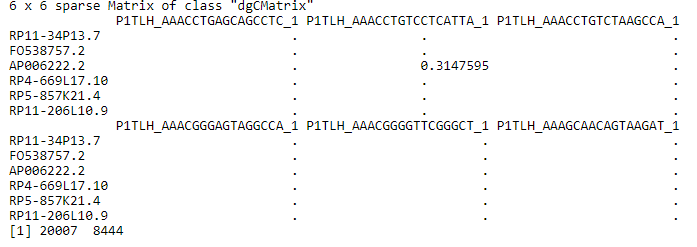
\includegraphics[width=9.68in]{livermatrix} 

}

\caption{First five rows and columns of the liver dataset}\label{fig:unnamed-chunk-4}
\end{figure}

Bone-Marrow Dataset: The bone marrow dataset is obtained from twenty
volunteers, that is, 10 males and 10 females with ages ranging from 24
to 84 years old and median age of 57 years. The scRNA-Seq (single cell
RNA- Sequencing) was performed using 10X Genomics Single Cell 3
Solution, version 2. Files from multiple donors were merged to obtain
the gene-expression matrix with row counts and the dimensions of the
matrix thus obtained were 33694 X 90653 and a seurat object was created
@ref\{Outline of Bioconductor Ecosystem\}. The dataset has 33694 genes
and 90653 cells which will be pre-processed and filtered for analysis.\\
The bone-marrow dataset used for analysis can be downloaded from :
\url{https://www.ncbi.nlm.nih.gov/geo/query/acc.cgi?acc=GSE120221}

\begin{figure}

{\centering 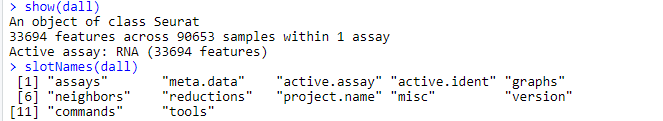
\includegraphics[width=9.21in]{bmobject} 

}

\caption{Seurat object created from gene-expression matrix of bone-marrow dataset}\label{fig:unnamed-chunk-5}
\end{figure}

\subsection{Challenges with Datasets:}\label{challenges-with-datasets}

The scRNA data is recorded at a single cell resolution, thus the size of
the count matrices may vary from The matrices used to store biological
information are large and working with these datasets is computationally
exhaustive. Therefore it is important to have good computational power
to carry out analysis using these datasets.To make it easier to work
with these datasets the information is stored using sparse matrices.
(?reference)

\subsection{Sparse Matrices}\label{sparse-matrices}

The matrices obtained from biological data are usually big and have many
zeros. Sparse matrices 5 are used when most of the elements in the
dataset are 0. Sparse Matrix saves a lot of space in the memory by
representing only the non-zero entries. It is computationally efficient
compared to the dense matrices and makes calculations faster. A matrix
is called dense when most of the elements in the matrix are non-zero.
The below example has been created using R {[}R{]} to understand the
advantages of sparse matrices compared to dense matrices.

\begin{figure}

{\centering 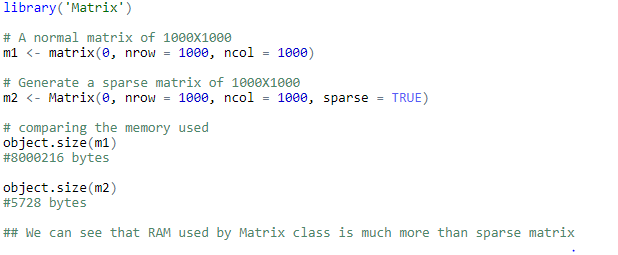
\includegraphics[width=8.58in]{Sparse1} 

}

\caption{Memory used in sparse and normal matrices}\label{fig:unnamed-chunk-6}
\end{figure}

If we add a single non-zero observation to the dataset we can clearly
see that space in memory occupied by the sparse matrix will increase
while the space occupied by the normal matrix will remain unchanged.

\begin{figure}

{\centering 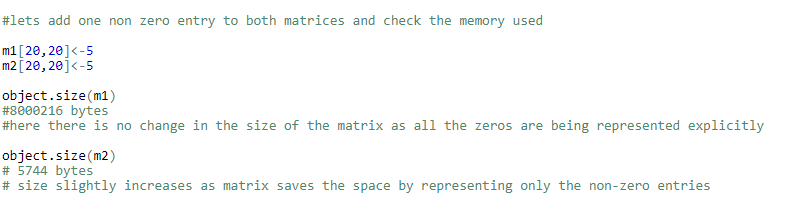
\includegraphics[width=10.92in]{Sparse2} 

}

\caption{Storage space for Sparse Matrices increase as they store the non-zero elements}\label{fig:unnamed-chunk-7}
\end{figure}

Both the datasets in this project have been stored as sparse matrix for
the ease of calculations.

\section{RNA-Sequencing Workflow}\label{rna-sequencing-workflow}

A typical RNA-Seq analysis consists of five steps. There are variety of
softwares and environments that can be used in the analysis of RNA-Seq
data, however the steps taken in an analysis workflow are typically
analogous and will follow the same procedure as discussed in this
project. The stages in the workflow are pre-processing of raw counts,
normalization, Dimensionality Reduction, Clustering and Labelling,
Differential Expression Analysis and Pathway Enrichment Analysis.Figure
\footnote{This image has been downloaded from \url{https://www.nature.com/articles/s41467-018-06318-7}[@macparland2018single]}
\ref{fig:rs} describes the workflow commonly used for analysing RNA-Seq
Data.

\begin{figure}[H]
  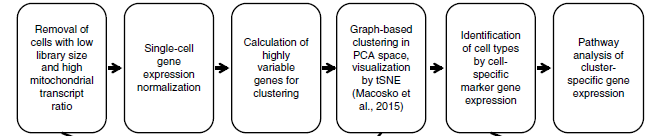
\includegraphics[scale=0.8]{rna-work.png}
  \caption{RNA-Seq Workflow}
  \label{fig:rs}
\end{figure}

The raw counts in the dataset are filtered to remove low quality and
dying cells. The resultant matrix is them normalized to make data
comparable and to prevent false biological
conclusions\autocite{steinhoff2006normalization}. Once, normalized
matrix is achieved then analysis is performed. Dimensionality reduction
techniques are used to reduce the number of genes (features) and to find
out important features. This is done with the help of various techniques
like Principal Component Analysis \autocite{jolliffe2011principal},
t-SNE \autocite{maaten2008visualizing}. Then clustering is done on the
results of PCA and the resultant clustered are labelled (refer chapter
4). The differentially expressed genes also known are marker genes are
then located (refer chapter 4).

\chapter{Outline of Bioconductor
Ecosystem}\label{outline-of-bioconductor-ecosystem}

Bioconductor is a collection of packages in R mainly used for genomics
study and analysis.

\section{Seurat object}\label{sec:seurat}

The analysis of the two datasets is conducted with the help of Seurat
Package version 3.0. Seurat is a toolkit for quality control, analysis,
and exploration of single cell RNA sequencing data. `Seurat' aims to
enable users to identify and interpret sources of heterogeneity from
single cell transcriptomic measurements, and to integrate diverse types
of single cell data. Seurat is developed and maintained by the Satija
lab \autocite{seurat}.

The Seurat package supports improved methods of normalization and
removes any variations that occur due to technical faults10. It provides
a flexible framework for multiple dataset integration and was used to
integrate various datasets for bone marrow data. Seurat has an advantage
in dealing with biological data as it automatically saves data as a
sparse matrix.\\
Seurat package stores all information of dataset and the analysis
results as a Seurat object.A Seurat object is created with the raw
counts which contains various slots which will store not only the raw
input data but also results from various computations. The function to
create a Seurat object is:

CreateSeuratObject(counts, project = ``SeuratProject'', assay = ``RNA'')

Here, the counts refer the unnormalized data such as raw counts and the
project sets name for the Seurat object and assay gives name of assay
corresponding to input data, in our case RNA.

A Seurat object named pbmc and dall were created for liver and
bonemarrow datasets respectivey. using package Seurat.
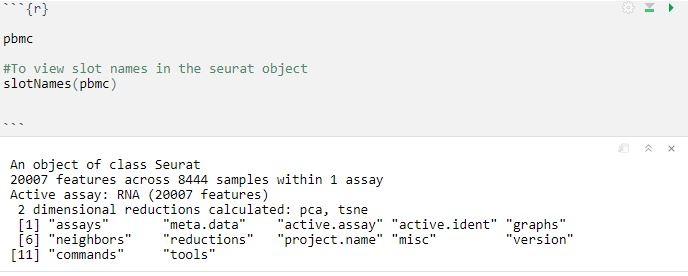
\includegraphics[scale=1.1]{seuratslots.JPG}

\chapter{Literature Review}\label{literature-review}

\chapter{METHODOLOGY}\label{ch:methods}

Analysis of scRNA datasets follows a similar pipeline for all datasets
however the computational functions used may vary from one package to
another. This section introduces the experimental design, describes
pre-processing workflow to obtain suitable data for analysis and
explains the various methods used for analysing the scRNA-seq datasets.

\section{Pre-Processing of Data}\label{sec:Pre-pro}

The new advancements in the field of health and medicine are dependent
on the data being analysed. It is essential to ensure the use of high
quality data to carry out such analysis. Data recorded for scRNA-seq
captures rna sequences in a cell using various sequencing technologies
\autocite{pareek2011sequencing}, but computational and technological
limitations often lead to capture of low quality data(improper or low
mRNA reads in a cell).\textcite{haque2017practical} reveals that even
with the high RNA-seq protocols some mRNA sequences were not captured in
the cell.To overcome this limitation,low quality cells are filtered
before analysis to ensure that technical effects do not distort the
downstream analysis results. The problematic cells which have low
library size and cell coverages are removed. A library is the total
number of reads aligned to each cell (total sum of counts across all
genes). Cell coverage is the average number of expressed genes in a
cell(average number of genes with non-zero counts). Low-quality / dying
cells often exhibit extensive mitochondrial contamination, therefore
cells with high mitochondrial genome transcript ratio are removed from
the dataset \ref{sec:Pre-pro}.

\subsection{Liver Dataset:}\label{liver-dataset}

The liver dataset was not filtered as normalized counts were already
provided. Cells with a very small library size (\textless{}1500) and a
very high (\textgreater{}0.5) mitochondrial genome transcript ratio were
already removed as High proportions are indicative of poor-quality cells
\autocite{ilicic2016classification} .The resulting dataset was then
normalised \ref{sec:norm} to get normalised
counts.\autocite[refer][]{macparland2018single}.

\subsection{Bonemarrow Dataset:}\label{bonemarrow-dataset}

The raw counts in the Bonemarrow dataset were processed and filtered to
remove the unwanted cells.Seurat object stores the number of UMIs
\footnote{Please refer to the document on  \url{https://www.illumina.com/science/sequencing-method-explorer/kits-and-arrays/umi.html} for more information on UMI}
\autocite{smith2017umi} per cell as nCount\_RNA, number of features per
cell as nFeature\_RNA and the fraction of mitochondrial RNA as
mt.percent in the metadata slot. The plot \ref{fig:fs} has been created
to visualize QC metrics and feature-feature relationships to find the
optimal cut-off value for filtering of cells.

\begin{figure}[H]
  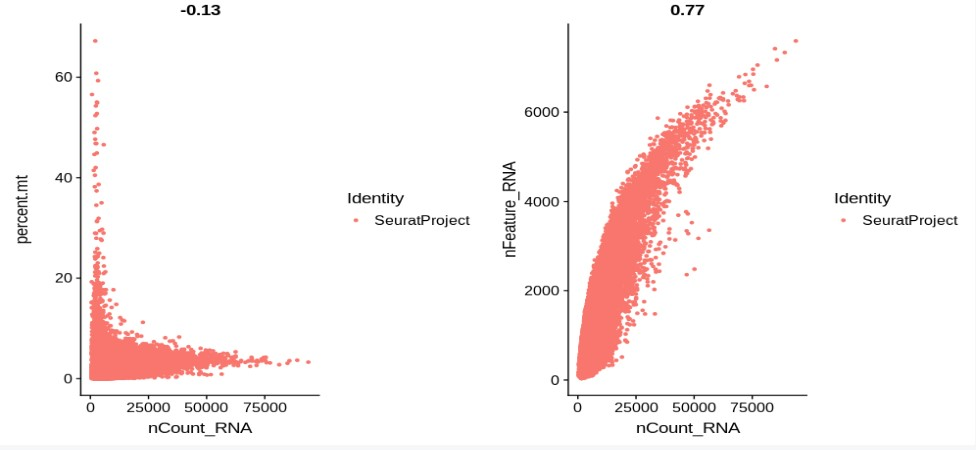
\includegraphics[scale=0.6]{featurescatter.jpg}
  \caption{Feature Scatter Plot}
  \label{fig:fs}
\end{figure}

Figure \ref{fig:fs} represents fraction of mitochondrial RNA (x-axis)
and number of features (x-axis) verses number of UMIs per cell (y-axis),
this plot assists in deciding optimum cutoff value for percent.mt and
nFeatureRNA. Cells with a very small library size (\textless{}500) and a
very high (\textgreater{}8\%) mitochondrial genome transcript ratio were
removed\autocite{ilicic2016classification}.After elimination of low
quality cells the remaining cells were used for analysis. Refer section
\ref{sec:bone}.

\section{Normalization of Data}\label{sec:norm}

After filtering of unwanted cells next step is to normalize the data.
Measurements from genetically distinct populations may occupy different
scales and to make them comparable normalization is performed. The
variance in the data tends to depend on the absolute intensity of the
data which may lead to false biological conclusions and should be
remedied by a normalization method \autocite{evans2017selecting}. By
default, Seurat\autocite{seurat} uses a global-scaling normalization
method ``Log Normalize'' that normalizes the gene expression
measurements for each cell by the total expression, multiplies this by a
scale factor (10,000 by default), and log-transforms the result
\autocite{cole2019performance}. The liver dataset already had normalized
counts and the bone marrow dataset was normalized using function
NormalizeData()
\footnote{For documentation please refer \url{https://rdrr.io/cran/Seurat/man/NormalizeData.html}}
in R\autocite{team2013r}.

\section{Finding Variable Genes}\label{sec:vg}

Variable features are identified after the data has been normalized.
Feature selection is an important step when dealing with large datasets
as it facilitates improved data quality and speeds up the procedure for
analysis \autocite{kursa2010feature}. Here, we will detect genes which
are highly variable. In the case of scRNA-seq data, the variation of
genes across cells can be a result of statistical noise rather than
biological factors\autocite{brennecke2013accounting}. Therefore, it
becomes important to identify the subset of genes whose variability in
the dataset exceeds the background of statistical noise.

To find highly variable genes (HVG), genes processing high biological
variations are targeted. Gene expression data may have
heteroscedasticity \autocite{yip2017linnorm}, thus variance cannot be
considered as the appropriate factor for determination of HVG.

FindVariableFeatures
\footnote{For documentation please refer \url{https://www.rdocumentation.org/packages/Seurat/versions/3.0.2/topics/FindVariableFeatures}}\label{refnote}
function in Seurat v3 uses the relationship between variance and mean as
the indicator of selecting HVG \autocite{yip2018evaluation}. The default
setting for selecting the HVG is method=``vst'' in which mean and
variance for each gene is calculated and then log-transformed. A loess
curve of polynomials of degree 2 is fit with a span of 0.3 to predict
the variance of each gene as a function of its mean. The values are then
standardised using the below transformation:

\[z_{ij}=\frac{{x_{ij}}-\bar{x}_i}{\sigma_i}\] where \(z_{ij}\) is the
standardized value of feature i in cell j, \(x_{ij}\) is the raw value
of feature i in cell j, \(\bar{x}_i\) is the mean raw value for feature
i, and \(\sigma_i\) is the expected standard deviation of feature
i.Then, the variance for all standardized values is computed across all
cells.\autocite{stuart2019comprehensive}.By default this function
selects 2000 genes but this number can be adjusted by the use of
argument ``nfeatures''\footref{refnote}.The results have been discussed
in section \ref{ch:results}

\section{Dimentionality Reduction}\label{sec:dm}

Genomics data records the activity of thousands of cell or genes which
makes the data larger. Larger datasets have computational limitations
and are more complex.Dimensionality reduction is important when the
number of features are more than the number of cases.Various
Dimensionality Reduction techniques like Principle Component Analysis
(PCA) \autocite{wold1987principal}, t-Distributed Stochastic Neighbor
Embedding (t-SNE) \autocite{maaten2008visualizing} and Uniform Manifold
Approximation and Projection (UMAP) \autocite{maaten2008visualizing}
were used to reduce the dimensions and project the data in lower
dimensions.This section describes the methodology used for performing
dimensionality reduction.

\subsection{Principle Component
Analysis}\label{principle-component-analysis}

PCA is a linear feature extraction un-supervised learning technique
widely for data with a high number of features
\autocite{wold1987principal}. It provides fully unsupervised information
on the dominant directions of highest variability in the data and can,
therefore, be used to investigate similarities between individual
samples, or formation of clusters \autocite{ringner2008principal}. PCA
performs linear mapping of the data to lower dimensional space so that
variance can be maximised which is done by calculating eigenvectors from
the covariance matrix. Eigenvectors that correspond to the largest
eigenvalues are used. \autocite{wold1987principal}.

The data selected containing the HVG is scaled prior to running PCA
using
ScaleData\footnote{\url{https://www.rdocumentation.org/packages/Seurat/versions/3.0.2/topics/ScaleData}}
function in Seurat v3.The ScaleData functions centres each feature to
have a mean of 0 and then scales it by the standard deviation of each
feature.

PCA is performed on the selected data using RunPCA
\footnote{\url{https://www.rdocumentation.org/packages/Seurat/versions/3.0.2/topics/RunPCA}}
function in Seurat v3 and the results are stored in the reductions slot
of Seurat Object.Results of PCA are discussed in section
\ref{sec:pcares}. The optimal number of Principal Components (PCs) are
picked using the
JackStraw\footnote{\url{https://www.rdocumentation.org/packages/Seurat/versions/3.0.2/topics/JackStraw}}
and
Elbow\textbackslash{}footnote\{\url{https://www.rdocumentation.org/packages/GMD/versions/0.3.3/topics/elbow}
Plots.

JackStraw Plot was used to determine the optimum number of principal
components for clustering.Jackstraw implements a resampling test
inspired by the JackStraw procedure. It randomly permutes a subset of
the data (1\% by default) and reruns PCA, constructing a `null
distribution' of feature scores and thus identifying statistically
significant PCs \autocite{chung2018jackstraw}.\\
The JackStraw Plot function
\footnote{\url{https://www.rdocumentation.org/packages/Seurat/versions/3.0.2/topics/JackStrawPlot}}
was used to visualize JackStraw results. Figure \ref{fig:figa}
demonstrates the distribution of p-values for each PC with a uniform
distribution (dashed line) and the PCs with curved lines above the
distribution are statistically significant PCs.

\begin{figure}[H]
  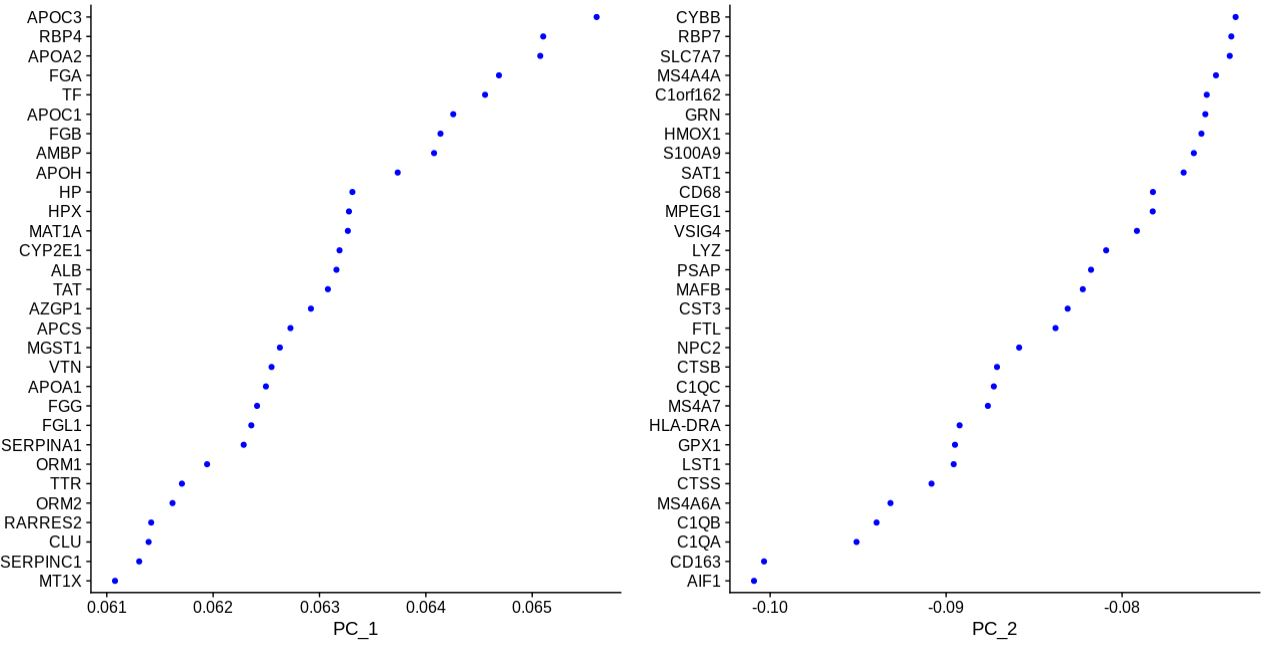
\includegraphics[scale=0.4]{pcloadliver.JPG}
  \caption{JackStaw Plot}
  \label{fig:figa}
\end{figure}

\subsection{t-SNE}\label{t-sne}

\section{Clustering of cells and
visualization}\label{clustering-of-cells-and-visualization}

\section{Differential Expression
Analysis}\label{differential-expression-analysis}

\section{Gene-coexpression analysis}\label{gene-coexpression-analysis}

\chapter{RESULTS (a)}\label{ch:results}

\textbf{Liver Dataset:}\\
The liver dataset was analysed and the samples were clustered to reveal
21 distinct cell populations in human liver. Differentially expressed
genes were calculated for each cluster and were studied to label each
cluster.Clusters with presence of senescence related profiles were
detected.Gene co-expression analysis was performed to find modules of
senescent associated genes.

\section{Highly Variable Genes}\label{sec:hvres}

The FindVariableFeatures \ref{sec:vg} function facilitated the selection
of 7000 HVG from normalized data.The selected HVG were used for PCA.

\begin{figure}[H]
  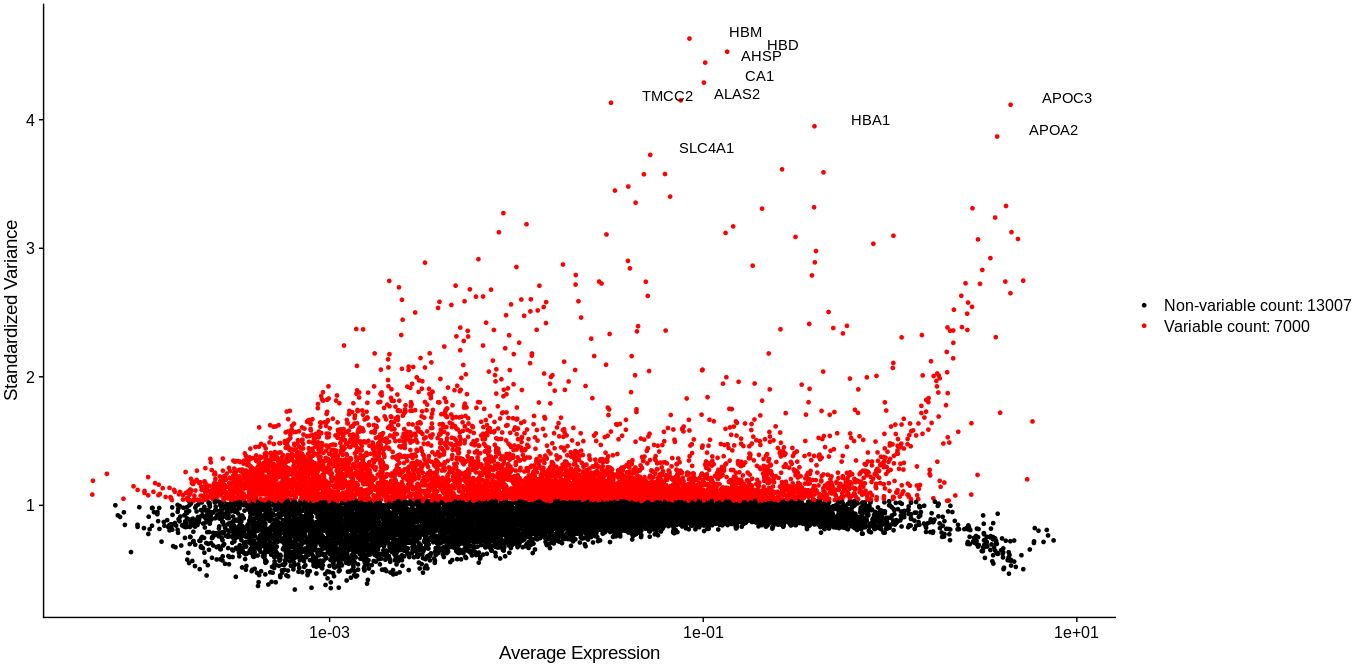
\includegraphics[scale=0.5]{hvgliver.JPG}
  \caption{Variable Genes Plot}
  \label{fig:fig1}
\end{figure}

Figure \ref{fig:fig1} labels the top 10 HVG and highlights HVG and the
genes which are non-variable.In the plot, X-axis function is the mean
expression level, and for Y-axis it is the log(Variance/mean).

\textit{Note:All mean/variance calculations are not performed in log-space, but the results are reported in log-space.\footnote{For documentation please refer \url{https://www.rdocumentation.org/packages/Seurat/versions/3.0.2/topics/FindVariableFeatures}}}

\section{Principal Component Analysis:}\label{sec:pcares}

After computation of HVG, the data was scaled The principal was
performed on variable genes and 50 principal components (PC) were
obtained.The first two principal components accounted for maximum
variability in the data.

\begin{figure}[H]
  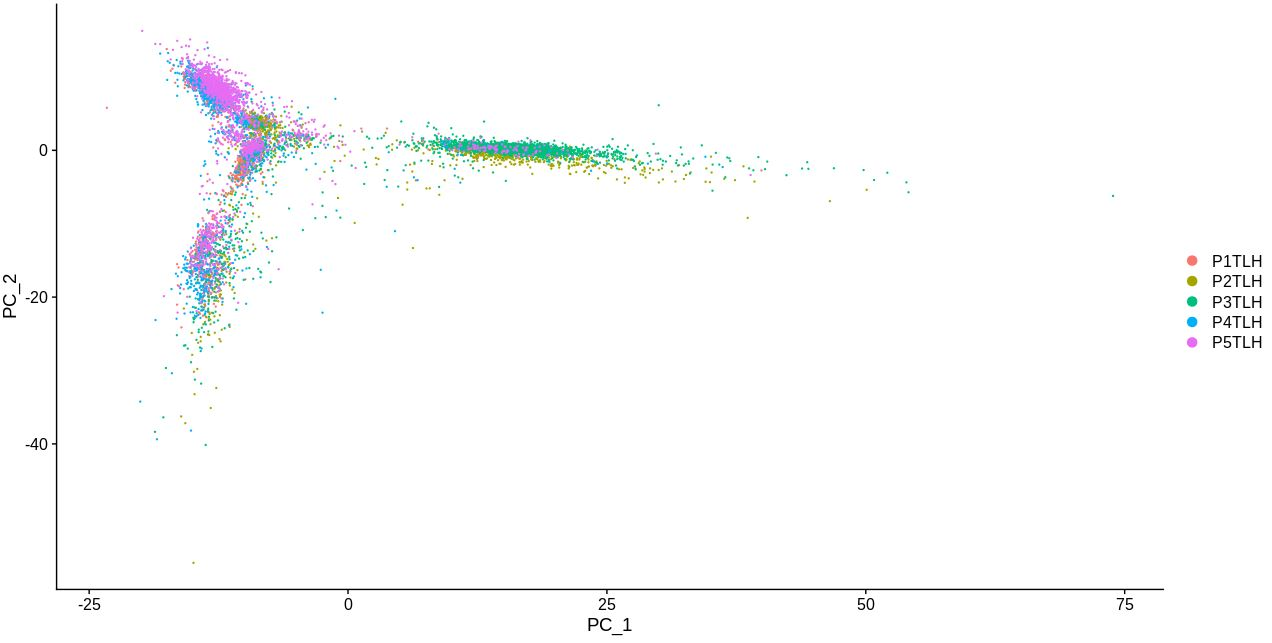
\includegraphics[scale=0.5]{pcaliver.JPG}
  \caption{Principal Component Plot of five samples}
  \label{fig:fig2}
\end{figure}

Figure \ref{fig:fig2} plots the first two principal components of the
samples.VizDimLoadings\footnote{https://www.rdocumentation.org/packages/Seurat/versions/3.0.2/topics/VizDimLoadings}
function in Seurat v3 can be used to visualize top genes associated with
principal components.

\begin{figure}[H]
  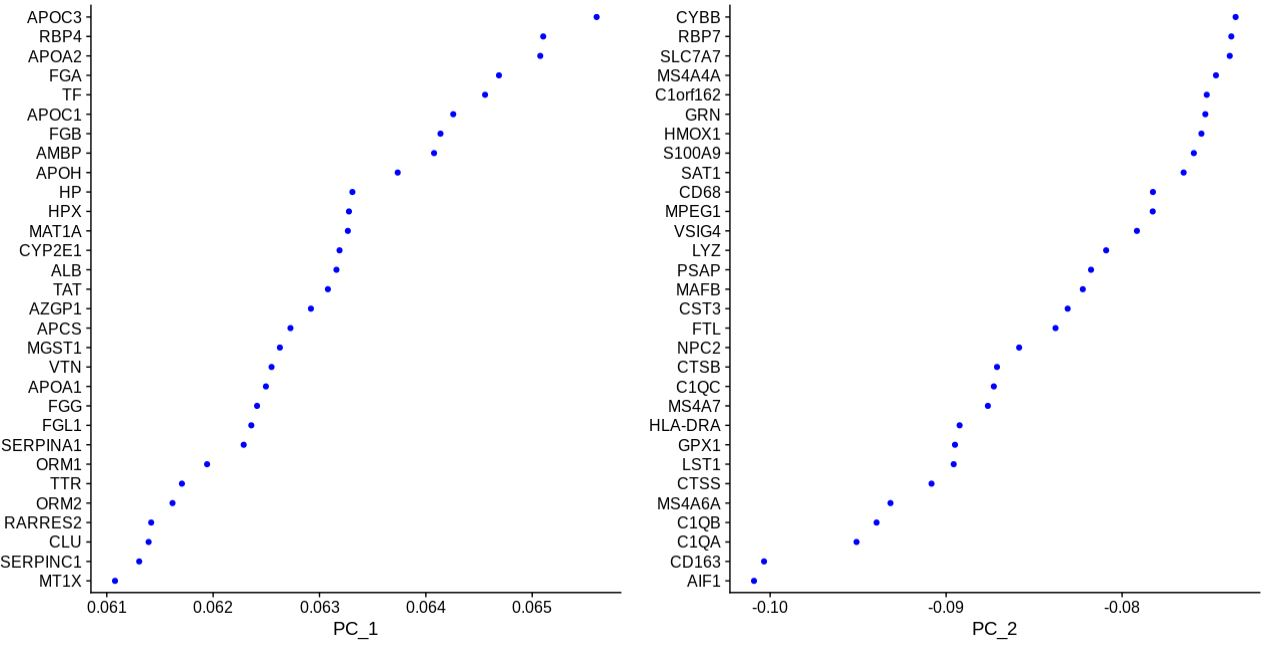
\includegraphics[scale=0.4]{pcloadliver.JPG}
  \caption{Loadings of PC1 and PC2}
  \label{fig:fig3}
\end{figure}

Figure \ref{fig:fig3} visualizes top genes associated with PC1 and PC2
with PC scores on x-axis and genes on y-axis. Larger absolute value of
component corresponds to a more important gene.

\chapter{RESULTS (b)}\label{ch:resultsb}

\textbf{Bonemarrow Dataset:}\\
The raw counts were filtered and the number of cells after removal of
low-quality cells was reduced to 76645 from 90653.Remaining 76645 cells
were used for final analysis.

\appendix

\chapter{Additional stuff}\label{additional-stuff}

You might put some computer output here, or maybe additional tables.

Note that \texttt{\textbackslash{}appendix} must appear before your
first appendix although this is not required for other appendices.

\chapter{Linear Mixed Model}\label{lmm}

The extension to the linear models is the linear mixed models. A general
form for the linear mixed model is given by

\begin{equation}
\boldsymbol{y} = \boldsymbol{X}\boldsymbol{\tau} + \boldsymbol{Z}\boldsymbol{u} + \boldsymbol{e} \label{eq:lmm}
\end{equation}

where \(\boldsymbol{y}\) is the \(n\times 1\) vector of observations on
the trait (or response) of interest, \(\boldsymbol{\tau}\) is a
\(p \times 1\) vector of fixed effects, \(\boldsymbol{u}\) is a
\(q \times 1\) vector of random effects, \(\boldsymbol{X}\) and
\(\boldsymbol{Z}\) are associated (known) design matrices specifying the
factors and covariates (explanatory variables) with corresponding fixed
and random effects vector respectively, and \(\boldsymbol{e}\) is the
\(n\times 1\) vector of errors. We assume that rank of
\(\boldsymbol{X}\) is \(p_0 < p\) (i.e.~non-full rank).

To complete the specification, we assume that the joint distribution of
\((\boldsymbol{u}, \boldsymbol{e})\) is \[ \begin{bmatrix}
\boldsymbol{u} \\
\boldsymbol{e} 
\end{bmatrix}
\sim N \left( 
\begin{bmatrix}
\boldsymbol{0} \\
\boldsymbol{0} 
\end{bmatrix}, 
\begin{bmatrix}
\boldsymbol{G} & \boldsymbol{0} \\
\boldsymbol{0} & \boldsymbol{R} 
\end{bmatrix}
\right)
\] where \(\boldsymbol{G}(\boldsymbol{\kappa_G})\) and
\(\boldsymbol{R}(\boldsymbol{\kappa_R})\) are covariance matrices which
depend on vectors \(\boldsymbol{\kappa_G}\) and
\(\boldsymbol{\kappa_R}\) respectively; and \(\theta\) is the global
scale parameter. We let
\(\boldsymbol{\kappa} = (\boldsymbol{\kappa_G}^\top, \boldsymbol{\kappa_R}^\top)^\top\)
denote the complete vectors of variance parameters.

It follows that
\(\boldsymbol{y} \sim N(\boldsymbol{X\tau}, \boldsymbol{V})\) where
\(\boldsymbol{V} = \boldsymbol{ZGZ}^\top + \boldsymbol{R}\) where
\(\boldsymbol{V}=\boldsymbol{V}(\boldsymbol{\kappa})\).

\printbibliography[heading=bibintoc]



\end{document}
